\documentclass[a4paper, 14pt]{extarticle}

% Поля
%--------------------------------------
\usepackage{geometry}
\geometry{a4paper,tmargin=2cm,bmargin=2cm,lmargin=3cm,rmargin=1cm}
%--------------------------------------


%Russian-specific packages
%--------------------------------------
\usepackage[T2A]{fontenc}
\usepackage[utf8]{inputenc}
\usepackage[english, main=russian]{babel}
%--------------------------------------

\usepackage{textcomp}

% Красная строка
%--------------------------------------
\usepackage{indentfirst}
%--------------------------------------


%Graphics
%--------------------------------------
\usepackage{graphicx}
\graphicspath{ {./images/} }
\usepackage{wrapfig}
%--------------------------------------

% Полуторный интервал
%--------------------------------------
\linespread{1.3}
%--------------------------------------

%Выравнивание и переносы
%--------------------------------------
\sloppy
\clubpenalty=10000
\widowpenalty=10000
%--------------------------------------

%Списки
\usepackage{enumitem}

%Подписи
\usepackage{caption}

%Гиперссылки
\usepackage{hyperref}

\hypersetup {
 unicode=true
}

%Рисунки
%--------------------------------------
\DeclareCaptionLabelSeparator*{emdash}{~--- }
\captionsetup[figure]{labelsep=emdash,font=onehalfspacing,position=bottom}
%--------------------------------------

\usepackage{tempora}

\usepackage{listings}
\usepackage{xcolor}

\lstset{
    basicstyle=\ttfamily,
    breaklines=true,
    columns=fullflexible,
    frame=single,
    inputencoding=utf8,
    extendedchars=true,
    keywordstyle=\bf,
    numbers=left,
    numbersep=5pt,
    xleftmargin=25pt,
    xrightmargin=25pt,
}


%--------------------------------------
%   НАЧАЛО ДОКУМЕНТА
%--------------------------------------

\begin{document}

%--------------------------------------
%   ТИТУЛЬНЫЙ ЛИСТ
%--------------------------------------
\begin{titlepage}
\thispagestyle{empty}
\newpage


%Шапка титульного листа
%--------------------------------------
\vspace*{-60pt}
\hspace{-65pt}
\begin{minipage}{0.3\textwidth}
\hspace*{-20pt}\centering

\includegraphics[width=\textwidth]{emblem}
\end{minipage}
\begin{minipage}{0.67\textwidth}\small \textbf{
\vspace*{-0.7ex}
\hspace*{-6pt}\centerline{Министерство науки и высшего образования Российской Федерации}
\vspace*{-0.7ex}
\centerline{Федеральное государственное бюджетное образовательное учреждение }
\vspace*{-0.7ex}
\centerline{высшего образования}
\vspace*{-0.7ex}
\centerline{<<Московский государственный технический университет}
\vspace*{-0.7ex}
\centerline{имени Н.Э. Баумана}
\vspace*{-0.7ex}
\centerline{(национальный исследовательский университет)>>}
\vspace*{-0.7ex}
\centerline{(МГТУ им. Н.Э. Баумана)}}
\end{minipage}
%--------------------------------------

%Полосы
%--------------------------------------
\vspace{-25pt}
\hspace{-35pt}\rule{\textwidth}{2.3pt}

\vspace*{-20.3pt}
\hspace{-35pt}\rule{\textwidth}{0.4pt}
%--------------------------------------

\vspace{1.5ex}
\hspace{-35pt} \noindent \small ФАКУЛЬТЕТ\hspace{80pt} <<Информатика и системы управления>>

\vspace*{-16pt}
\hspace{47pt}\rule{0.83\textwidth}{0.4pt}

\vspace{0.5ex}
\hspace{-35pt} \noindent \small КАФЕДРА\hspace{50pt} <<Теоретическая информатика и компьютерные технологии>>

\vspace*{-16pt}
\hspace{30pt}\rule{0.866\textwidth}{0.4pt}

\vspace{11em}

\begin{center}
\Large {\bf Лабораторная работа № 2} \\

\large {\bf по курсу <<Базы данных>>} \\[0.8cm]

\large <<Моделирование данных с использованием модели\\
семантических объектов>>
\end{center}
\normalsize

\vspace{8em}


\begin{flushright}
  {Студент группы ИУ9-51Б Хромов М.А. \hspace*{15pt}\\
  \vspace{2ex}
  Преподаватель Вишняков И. Э.\hspace*{15pt}}
\end{flushright}

\bigskip

\vfill


\begin{center}
\textsl{Москва 2026}
\end{center}
\end{titlepage}


% =================================================
% ОСНОВНАЯ ЧАСТЬ
% =================================================

\setcounter{page}{2}

\section{Задача}

\begin{enumerate}
  \item Создать модель семантических объектов для предметной области, выбранной в лабораторной работе № 1.
  \item Обосновать выбор кардинальных чисел атрибутов и типов объектов.
\end{enumerate}

\section{Практическая реализация}

\subsection{Предметная область}
\label{subsec:subject}

Предметная область <<Турнирный оператор>> включает учёт киберспортивных турниров, команд и результатов их участия. Приняты следующие требования:

\begin{itemize}
  \item Каждый турнир проводится одним организатором по одной дисциплине. Организатор и дисциплина могут быть связаны с несколькими турнирами.
  \item Турнир однозначно определяется организатором, дисциплиной, названием серии и датой начала.
  \item В турнире могут участвовать несколько команд, а команда может участвовать в нескольких турнирах. В пределах одного турнира каждая команда учитывается не более одного раза.
  \item Сведения об участии хранятся внутри турнира: команда, дата регистрации, статус, итоговое место и призовые. Дата регистрации и статус обязательны; результаты могут отсутствовать до их определения.
  \item Организаторы, дисциплины и команды могут быть зарегистрированы до появления связанных турниров. Турнир может быть создан до регистрации участников.
  \item Названия организаторов, дисциплин и команд уникальны в пределах соответствующих классов объектов.
\end{itemize}

\subsection{Построение модели семантических объектов}
\label{subsec:model}

Кардинальные числа парных объектных атрибутов согласованы следующим образом:

\subsubsection{Организатор}

\textbf{Организатор}. Идентификатор -- \textbf{Название организатора} (1.1). Простые атрибуты:
  \begin{itemize}
    \item Страна -- 1.1;
    \item Сайт -- 0.1;
    \item Контактный email -- 1.1.
  \end{itemize}
  Объектный атрибут: \textbf{Турнир} -- 0.N.

\textbf{Организатор -- Турнир:} организатор связан с 0.N турнирами; каждый турнир имеет одного организатора (1.1).

\textbf{Организатор} -- сложный объект: содержит объектный атрибут \textbf{Турнир}.

\subsubsection{Турнир}

\textbf{Турнир}. Составной идентификатор: \textbf{Название серии}, \textbf{Дата начала}, объектные атрибуты \textbf{Организатор} и \textbf{Дисциплина}. Кардинальность каждого компонента -- 1.1. Простые атрибуты вне идентификатора:
  \begin{itemize}
    \item Дата окончания -- 1.1;
    \item Призовой фонд -- 1.1;
    \item Формат -- 1.1.
  \end{itemize}
  Групповой атрибут \textbf{Участие в турнире} имеет кардинальность 0.N и содержит:
  \begin{itemize}
    \item Команда -- объектный атрибут с кардинальностью 1.1;
    \item Дата регистрации -- 1.1;
    \item Статус -- 1.1;
    \item Итоговое место -- 0.1;
    \item Призовые -- 0.1.
  \end{itemize}
  Маркер ID у атрибута \textbf{Команда} запрещает повторение одной команды в группе \textbf{Участие в турнире} в пределах конкретного турнира. Ссылка на сам турнир внутри группы не требуется: он определяется её принадлежностью объекту.

Группа \textbf{Идентификатор турнира} имеет кардинальность 1.1: у турнира один набор идентифицирующих компонентов. Уникальность относится ко всей комбинации. Группа \textbf{Участие в турнире} имеет кардинальность 0.N: для каждой участвующей команды создаётся отдельный экземпляр группы со своими результатами.

\textbf{Турнир} -- гибридный объект: содержит многозначную группу \textbf{Участие в турнире}, объединяющую объектный атрибут \textbf{Команда} и простые атрибуты регистрации и результатов.

\textbf{Участие в турнире} является групповым атрибутом, а не самостоятельным семантическим объектом. Дата регистрации, статус, место и призовые относятся к конкретной команде в конкретном турнире и хранятся вместе в одном экземпляре группы.

\subsubsection{Дисциплина}

\textbf{Дисциплина}. Идентификатор -- \textbf{Название дисциплины} (1.1). Простые атрибуты:
  \begin{itemize}
    \item Жанр -- 1.1;
    \item Разработчик -- 1.1.
  \end{itemize}
  Объектный атрибут: \textbf{Турнир} -- 0.N.

\textbf{Дисциплина -- Турнир:} дисциплина связана с 0.N турнирами; каждый турнир относится к одной дисциплине (1.1).

\textbf{Дисциплина} -- сложный объект: содержит объектный атрибут \textbf{Турнир}.

\subsubsection{Команда}

\textbf{Команда}. Идентификатор -- \textbf{Название команды} (1.1). Простые атрибуты:
  \begin{itemize}
    \item Тег -- 1.1;
    \item Страна -- 1.1;
    \item Дата создания -- 0.1.
  \end{itemize}
  Объектный атрибут: \textbf{Турнир} -- 0.N.

\textbf{Турнир -- Команда:} турнир содержит 0.N экземпляров группы участия, в каждом из которых указана одна команда (1.1). Обратный атрибут \textbf{Турнир} у команды имеет кардинальность 0.N. Так представлена связь <<многие-ко-многим>>.

\textbf{Команда} -- сложный объект: содержит объектный атрибут \textbf{Турнир}.

\begin{figure}[ht]
  \centering
  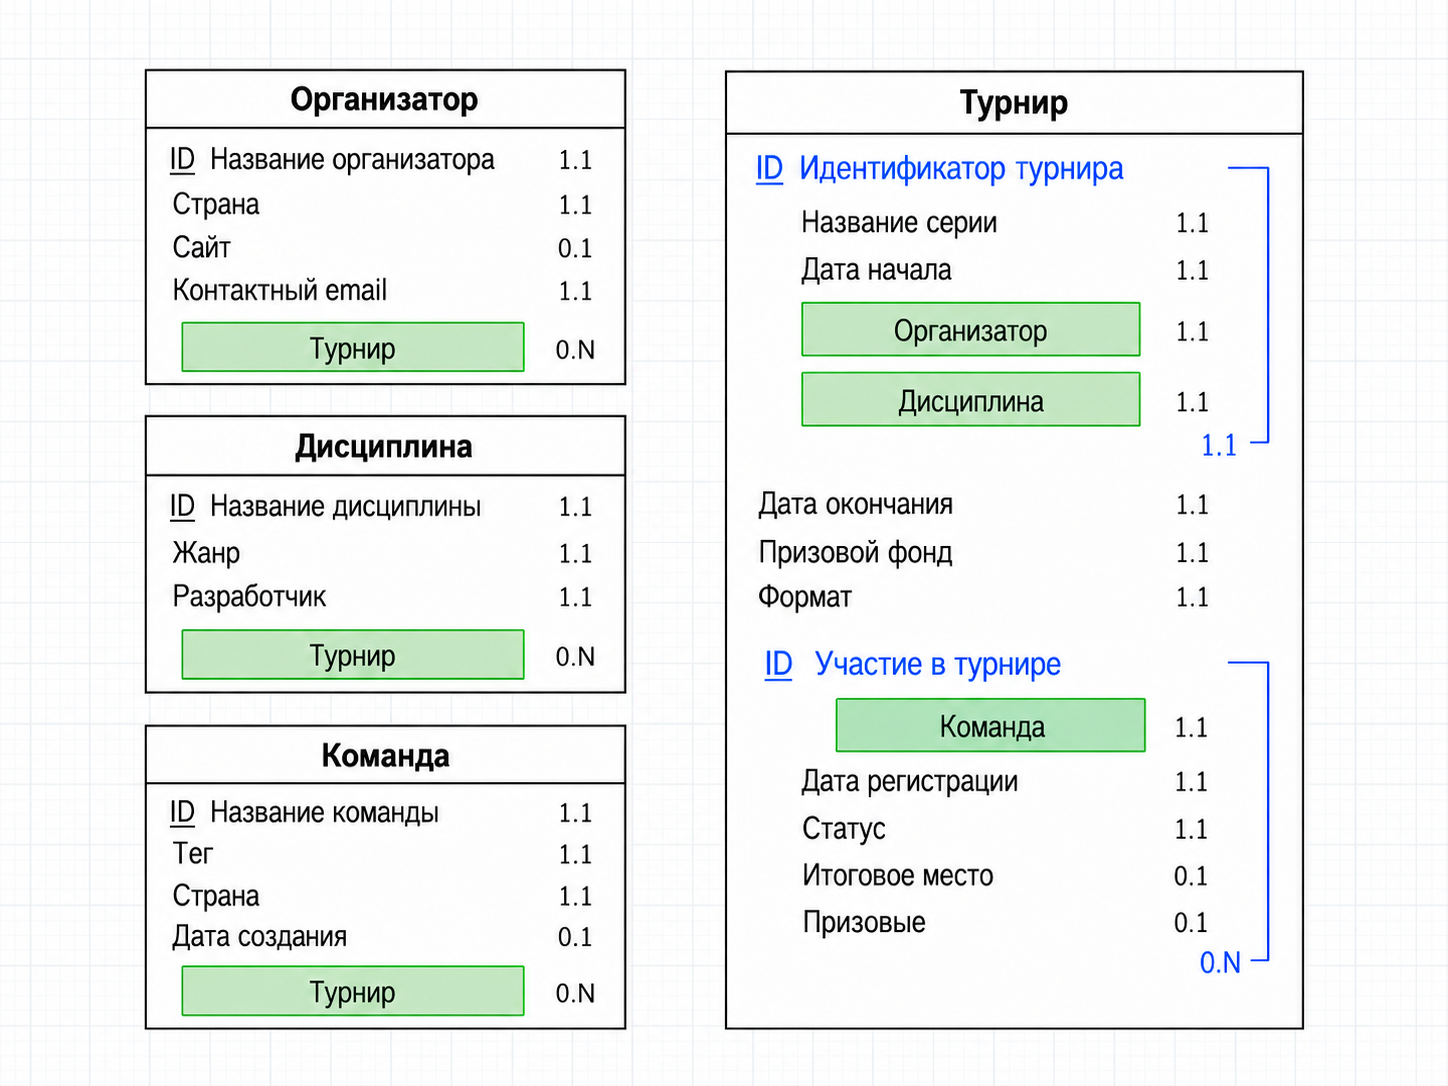
\includegraphics[width=0.9\textwidth]{labdb2.png}
  \caption{Модель семантических объектов}
  \label{fig:semantic-model}
\end{figure}


\end{document}
